% !TEX TS-program = pdflatex
% !TEX encoding = UTF-8 Unicode

% This is a simple template for a LaTeX document using the "article" class.
% See "book", "report", "letter" for other types of document.

\documentclass[11pt]{article} % use larger type; default would be 10pt

\usepackage[english]{babel}
\usepackage[utf8]{inputenc} % set input encoding (not needed with XeLaTeX)
\usepackage{fvextra}
\usepackage{csquotes}

%%% Examples of Article customizations
% These packages are optional, depending whether you want the features they provide.
% See the LaTeX Companion or other references for full information.

%%% PAGE DIMENSIONS
\usepackage[a4paper, top=2cm, bottom=2.2cm, left=3cm, right=3cm, includeheadfoot, headheight=31pt,
  headsep=0pt]{geometry} % to change the page dimensions
\geometry{a4paper} % or letterpaper (US) or a5paper or....
\usepackage{multicol}
\setlength{\headheight}{35pt}
\setlength{\parindent}{0pt}
% \geometry{landscape} % set up the page for landscape
%   read geometry.pdf for detailed page layout information

\usepackage{graphicx} % support the \includegraphics command and options
\usepackage[colorlinks=true, allcolors=blue]{hyperref}
\usepackage{xcolor} % Allow coloring of text.

% \usepackage[parfill]{parskip} % Activate to begin paragraphs with an empty line rather than an indent

%%% PACKAGES
\usepackage{booktabs} % for much better looking tables
\usepackage{array} % for better arrays (eg matrices) in maths
\usepackage{paralist} % very flexible & customisable lists (eg. enumerate/itemize, etc.)
\usepackage{fancyvrb} % adds environment for commenting out blocks of text & for better verbatim
\usepackage{subfig} % make it possible to include more than one captioned figure/table in a single float
\usepackage{float}
\usepackage{biblatex}[style=ieeetr]
\usepackage{parskip}
\usepackage{amsmath, amsthm, amssymb, amsfonts}
\usepackage{lipsum}
\usepackage{tabularx}
\usepackage[most]{tcolorbox}
\usepackage{calculator}
% These packages are all incorporated in the memoir class to one degree or another...

% Changes date format to YYYY-MM-DD
\usepackage[yyyymmdd]{datetime}
\settimeformat{hhmmsstime}
\renewcommand{\dateseparator}{-}

% Add version number variable.
\newcounter{versionNumber}
\makeatletter
% At the end write the current value back to the `.aux` file
\AtEndDocument{
  \immediate\write\@auxout{
    \string\setcounter{versionNumber}{\number\value{versionNumber}}
  }
}
\makeatother
% Step the counter at the beginning
\AtBeginDocument{
  \stepcounter{versionNumber}
}

% Title page info
\title{Rotating Index Load Balancer Documentation}
\author{Lani Wagner\\\href{mailto:lani.wagner@students.fhnw.ch}{lani.wagner@students.fhnw.ch}}
\date{\today\ \currenttime} % Activate to display a given date or no
% otherwise the current date is printed

% Define constants to use throughout document
\makeatletter
\let\thisauthor\@author
\makeatother

%%% HEADERS & FOOTERS
\usepackage{lastpage}
\usepackage{fancyhdr} % This should be set AFTER setting up the page geometry
\pagestyle{fancy} % options: empty , plain , fancy
\renewcommand{\headrulewidth}{0pt} % customise the layout...
\lhead{}
\chead{}
\rhead{
\includegraphics[height=0.88\headheight]{res/fhnw_ht_10mm.eps}}
\lfoot{v1.0.\theversionNumber\ \textcolor{gray}{\today\ \currenttime}}
\cfoot{Lani Wagner}
\rfoot{\thepage\ /
    {\hypersetup{hidelinks}\pageref{LastPage}}}

%%% SECTION TITLE APPEARANCE
\usepackage{sectsty}
\allsectionsfont{\sffamily\mdseries\upshape} % (See the fntguide.pdf for font help)
% (This matches ConTeXt defaults)

%%% ToC (table of contents) APPEARANCE
\usepackage[nottoc]{tocbibind} % Put the bibliography in the ToC
\usepackage[titles,subfigure]{tocloft}
\usepackage{amssymb} % Alter the style of the Table of Contents
\renewcommand{\cftsecfont}{\rmfamily\mdseries\upshape}
\renewcommand{\cftsecpagefont}{\rmfamily\mdseries\upshape} % No bold!

% Change second level of enumerated lists to arabic numbers.
\renewcommand{\labelenumii}{\arabic{enumi}.\arabic{enumii}}

% Reduce spacing in whole document to compact document
\usepackage{titlesec}
\usepackage{amsfonts}
\usepackage{enumitem}% http://ctan.org/pkg/enumitem
\setlist[itemize]{noitemsep, topsep=0pt}

\newcommand{\rilb}{Rotating Index Load Balancer}
\newcommand{\hidelinks}[1]{{\hypersetup{hidelinks}#1}}
\newcommand{\figref}[1]{\hidelinks{\hyperref[#1]{Figure \ref{#1}}}}
\newcommand{\ai}[1]{\textcolor{red}{$A_1$}}
\newcommand{\aii}[1]{\textcolor{green!50!black}{$A_2$}}
\newcommand{\aiii}[1]{\textcolor{blue!70!black}{$A_3$}}
\newcommand{\fn}[1]{\tcbox[on line, boxsep=0pt, arc=1pt, outer arc=1pt,
  left=1pt,
  right=1pt,
  top=0pt,
  bottom=0pt, colback=black!15!white, colframe=white]{#1}}

%%% END Article customizations

%%% The "real" document content comes below...

\begin{document}
  \begin{titlepage}
    \begin{center}
      \vspace*{1cm}

      \textbf{\Huge \rilb}

      \vspace{1.5cm}
      \hrule
      \vspace{1cm}

      {\Large Documentation}

      \vspace{2.5cm}


      \begin{figure}[H]
        \centering
        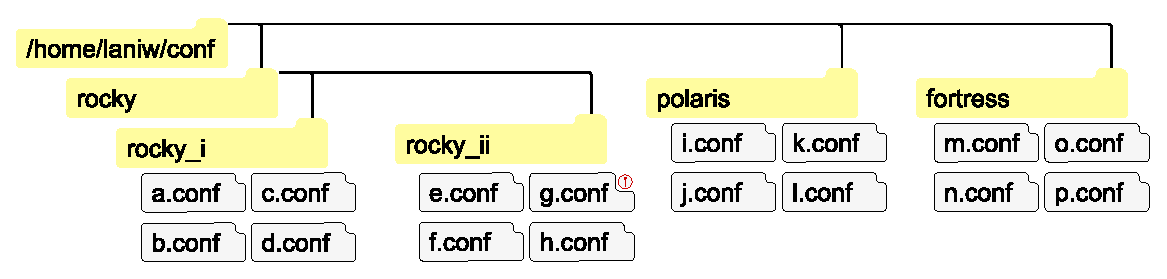
\includegraphics[width=.9\linewidth, keepaspectratio]{res/rilb_visualization}
        \label{fig:rilb-vis-title}
      \end{figure}

      \vfill

      
\includegraphics[width=0.4\textwidth]{res/fhnw_ht_10mm}

      \vspace{0.8cm}

      Lani Wagner

      \today\ \currenttime

    \end{center}
  \end{titlepage}

  \section*{Introduction}

  This document serves as a documentation for the written implementation of a rotating index load balancer as described in the pre-production specification found at \url{https://github.com/laniwfhnw/engw_specification/blob/main/engw_specification.pdf}.

    {\hypersetup{hidelinks} \tableofcontents}
  \newpage



  \section{\rilb{} Concept}\label{sec:2}

  To explain what the idea of a \rilb{} is, it's easiest to first explain what problem it solves with a simple example. Imagine a filesystem like the one shown in \figref{fig:rilb-vis}. We want to provide a service that accepts analysis requests. These analysis requests are run over the system to calculate a result. The result is then returned to the requester. You can imagine this service being an API, so we don't know when or how many of the requests we're going to get.

  The simplest solution, once we get a request, would be to go through all of the files for one request and complete the analysis. Once all of the files have been included in the result we return the result. This works fine when we don't have many requests coming in and the analyses don't need a long time to complete. We are doing a lot of the same operations multiple times, though. Every time we read a file for one analysis and then another and then another we are performing the same operation. If the analysis requests come in at a similar time, we can read the file once to avoid expensive I/O operations.

  The idea of reducing the amount of read operations $m \cdot n$ (where $m$ is the number of analyses that each need to read $n$ files) to $n$ read operations is the main idea of a \rilb{}. Imagine an index that points to a file at all times, and that can rotate and point to all files in the filesystem. Every time it points to a file it reads that file and passes that data on to all the analyses. Once a request for an anlysis reaches the service, the service keeps track of the first file that analysis received. The service knows that the analysis has looked at all files when the index once again points to the file that the analysis started with.

  \begin{figure}[H]
    \centering
    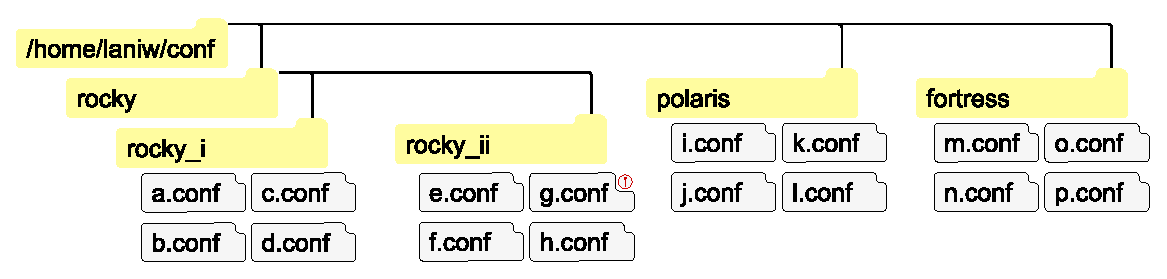
\includegraphics[width=.99\linewidth, keepaspectratio]{res/rilb_visualization}
    \caption{Visualization of a \newcommand{\ai}[1]{\textcolor{red}{#1}}{} traversion through an example filesystem.}
    \label{fig:rilb-vis}
  \end{figure}

  Let me me walk you through an example execution using the filesystem in \figref{fig:rilb-vis}. We are working with 16 different configuration files. We want to analyze these files in three different ways. The first analysis \ai{} determines the average length of the files (in lines). The second analysis \aii{} determines the longest line in any of the files. Finally, the third analysis \aiii{} determines the size of those files (in bytes) that are two levels deeper than the root. At first the service isn't doing anything because there are no active analyses running. Once the first analysis \ai{} is requested, the index starts rotating and the file contents are analysed in \ai{}. The files \fn{a.conf}, \fn{b.conf}, \fn{c.conf}, and \fn{d.conf} are analysed without any other requests coming in. The request for analysis \aii{} reaches the service right before the index points to \fn{e.conf}, so \fn{e.conf} is the first file \aii{} analyses. \aiii{} comes in when the
  index points to \fn{g.conf}. The contents of \fn{g.conf} and \fn{h.conf} are sent to all three analyses. The files \fn{i.conf} through \fn{p.conf} are only sent to analyses \ai{} and \aii, since analysis \aiii{} doesn't care about those files. As soon as the index points to \fn{a.conf} the second time the service knows that analysis \ai{} has been completed and it returns the result. The rotation continues without interruption until the index points to \fn{e.conf}, at which point the result of analysis \aii{} is returned. Now only analysis \aiii{} remains. It is still in the queue and receives the file contents of \fn{e.conf} and \fn{f.conf}. The result of analysis \aiii{} is returned as soon as the index points to \fn{g.conf}. Now there are no more analyses in the queue, so the index rests at \fn{g.conf} until another request arrives. The final state of the service is depicted in \figref{fig:rilb-vis}.

  This example obviously doesn't illustrate what happens in certain special cases. For example we didn't consider the case that \fn{g.conf} could get deleted during the rotation of \aiii, so with our current approach we would not know when to stop. For more detail on the exact implementation and how special cases are handled please take a look at the pre-production specification of the library\footnote{\url{https://github.com/laniwfhnw/engw_specification/blob/main/engw_specification.pdf}\label{fn:pp-spec}}.



  \section{Library Use}\label{sec:3}

  For a detailed description of the library interface please take a look at chapter two (``Design'') of the \rilb{} pre-production specificiation\hyperref[fn:pp-spec]{\footnotemark[1]}.


  \subsection{Environment}\label{sec:3.1}

  Since this library is written in Java it can run on any operating system that can run the JVM. This library is ideally suited to run on a system with multiple cores. Every analysis can run on a separate thread as soon as the file contents of the current file have been loaded into memory. Ideally you would provide a system with as many cores as you have analyses running on that system. For the ideal execution time you want to run this library on a system with enough RAM to run the application itself, hold the result of analyses and the largest file in the filesystem that the analyses are supposed to analyze.


  \subsection{Use Cases}\label{sec:3.2}

  This library is very well suited for a service that receives a lot of requests that need to analyze the same files over and over and over again with slightly different parameters each time. It can also be used in a very volatile filesystem (where file are getting deleted and created very regularly) although the accuracy of rotation completion and a little bit of performance will have to be sacrificed.

  Absolutely no guarantees are made about the performance of this library. It is the responsibility of the developer implementing this technology to verify whether the use is appropriate.



  \newpage



  \section{Glossary}

  \begin{table}[H]
    \centering
    \begin{tabular}{p{.3\linewidth} | p{.6\linewidth}}
      \textbf{Term} & \textbf{Definition}
      \\\hline
      Rotation            & A single go around the list of files considered for analysis.                                                      \\\hline
      Rotation completion & Using the first file an analysis receives as the indication that all files in the filesystem have been considered.
    \end{tabular}
    \caption{Glossary definitions.}
    \label{tab:glossary}
  \end{table}

  \printbibliography[heading=bibintoc]
  \listoffigures
  \listoftables
\end{document}